\documentclass[11pt]{article}
\usepackage[utf8]{inputenc}
\usepackage[T1]{fontenc}
\usepackage{lmodern}
\usepackage{geometry}
\usepackage{tikz}
\usetikzlibrary{arrows.meta,shapes.geometric}

\geometry{paperwidth=16cm,paperheight=7.4cm,margin=0cm}
\pagestyle{empty}
\setlength{\parindent}{0pt}

\definecolor{ctxFill}{RGB}{238,242,245}
\definecolor{ctxLine}{RGB}{155,168,179}
\definecolor{ctxText}{RGB}{38,52,67}
\definecolor{exFill}{RGB}{220,233,247}
\definecolor{exLine}{RGB}{23,54,93}
\definecolor{prFill}{RGB}{200,240,236}
\definecolor{prLine}{RGB}{8,127,140}
\definecolor{prText}{RGB}{6,79,87}
\definecolor{phFill}{RGB}{234,242,245}

\begin{document}
\noindent
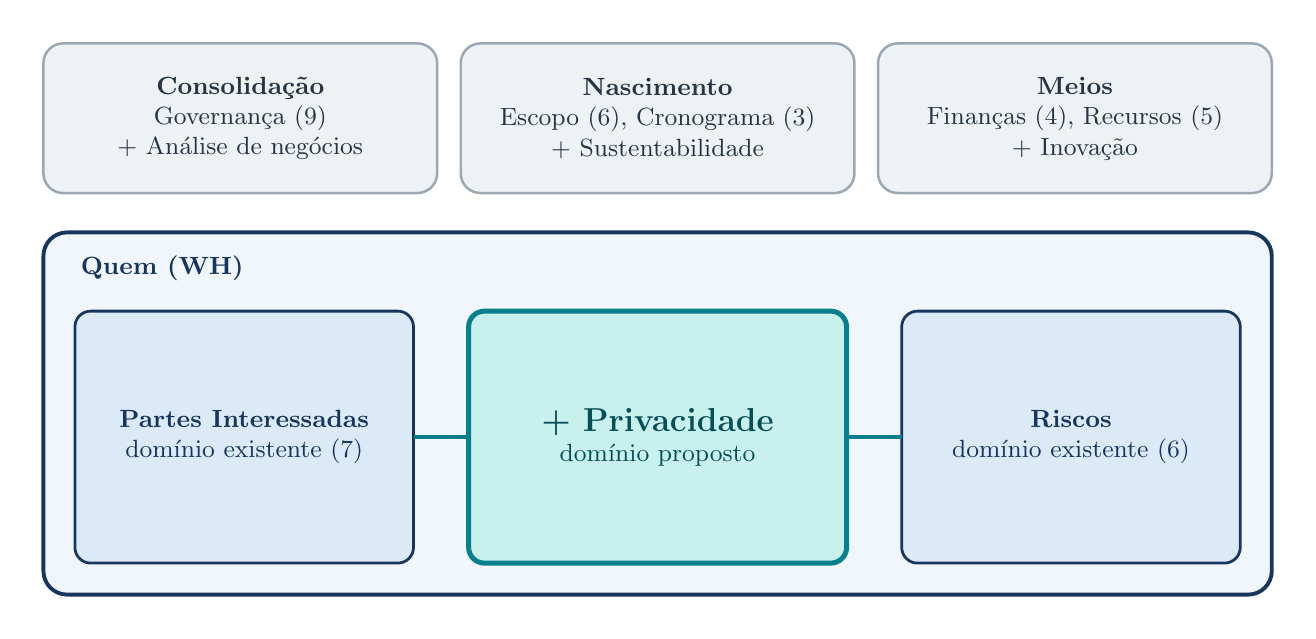
\begin{tikzpicture}[x=1cm,y=1cm,font=\small]
  \path[use as bounding box] (0,0) rectangle (16,7.4);
  \draw[fill=ctxFill,draw=ctxLine,line width=0.9pt,rounded corners=0.25cm] (0.2,5.3) rectangle (5.2,7.2);
  \node[align=center,text=ctxText] at (2.7,6.25) {\textbf{Consolidação}\\ Governança (9)\\+ Análise de negócios};
  \draw[fill=ctxFill,draw=ctxLine,line width=0.9pt,rounded corners=0.25cm] (5.5,5.3) rectangle (10.5,7.2);
  \node[align=center,text=ctxText] at (8.0,6.25) {\textbf{Nascimento}\\ Escopo (6), Cronograma (3)\\+ Sustentabilidade};
  \draw[fill=ctxFill,draw=ctxLine,line width=0.9pt,rounded corners=0.25cm] (10.8,5.3) rectangle (15.8,7.2);
  \node[align=center,text=ctxText] at (13.3,6.25) {\textbf{Meios}\\ Finanças (4), Recursos (5)\\+ Inovação};
  \draw[fill=exFill!40,draw=exLine,line width=1.4pt,rounded corners=0.3cm] (0.2,0.2) rectangle (15.8,4.8);
  \node[anchor=west,text=exLine] at (0.55,4.35) {\textbf{Quem (WH)}};
  \draw[fill=exFill,draw=exLine,line width=1pt,rounded corners=0.2cm] (0.6,0.6) rectangle (4.9,3.8);
  \draw[fill=prFill,draw=prLine,line width=1.8pt,rounded corners=0.2cm] (5.6,0.6) rectangle (10.4,3.8);
  \draw[fill=exFill,draw=exLine,line width=1pt,rounded corners=0.2cm] (11.1,0.6) rectangle (15.4,3.8);
  \node[align=center,text=exLine] at (2.75,2.2) {\textbf{Partes Interessadas}\\ domínio existente (7)};
  \node[align=center,text=prText] at (8.0,2.2) {\large\textbf{+ Privacidade}\\ domínio proposto};
  \node[align=center,text=exLine] at (13.25,2.2) {\textbf{Riscos}\\ domínio existente (6)};
  \draw[draw=prLine,line width=1.2pt] (4.9,2.2) -- (5.6,2.2);
  \draw[draw=prLine,line width=1.2pt] (10.4,2.2) -- (11.1,2.2);
\end{tikzpicture}
\end{document}
